

\iffalse
% This is LLNCS.DEM the demonstration file of
% the LaTeX macro package from Springer-Verlag
% for Lecture Notes in Computer Science,
% version 2.4 for LaTeX2e as of 16. April 2010
%
\documentclass[12pt]{llncs}
\usepackage{iftex}
\usepackage{nla}
%\usepackage{showframe}
%
%
\begin{document}
\fi

\title{Optimization of the solutions of the pseudogeometric version of the traveling salesman problem}
%
\titlerunning{Hamiltonian Mechanics}  % abbreviated title (for running head)
%                                     also used for the TOC unless
%                                     \toctitle is used
%
\author{%
Boris Melnikov\inst{1}
\and
Elena Melnikova\inst{2}
}
%
\authorrunning{Boris Melnikov and Elena Melnikova} % abbreviated author list (for running head)
%
%%%% list of authors for the TOC (use if author list has to be modified)
\tocauthor{Boris Melnikov and Elena Melnikova}
%
\institute{Shenzhen MSU\,--\,BIT University,
International University Park Road, Shenzhen, 518172, China,
\email{bormel@mail.ru}
\and
Russian State Social University,
No. 4, Wilhelm Pieck str., Moscow, 129226, Russia,
\email{ya.e.melnikova@yandex.ru}}

\maketitle              % typeset the title of the contribution

\begin{abstract}
We continue to consider the pseudogeometric version of the traveling salesman problem. 
At the same time, we propose our own version of the "onion husk" algorithm, which, unlike its usual descriptions, is oriented not to a geometric variant, but to a pseudo-geometric one.
We also describe our own version of random data generation for computational experiments, and we consider this option adequate for most real models.
For each of the several variants of the problem dimension, we conducted some computational experiments with randomly generated input data. 
The obtained results of computational experiments generally approximately corresponded to the expected values.
\keywords{
optimization problems, traveling salesman problem, Hamilton cycles, 
heuristic algorithms}
\end{abstract}

%%%%%%%%%%%%%%%%%%%%%%%%%%%%%%%%%%%%%%%%%%%%%%%%%%%%%%%%%%%%%%%%
In this paper, 
we continue to consider the pseudogeometric version 
of the traveling salesman problem, 
\cite{gu-pu,KIO-2021,KIO-2022,Vasil-2022-1,Vasil-2022-2,SOI-2013}.
We compared the total length of the contours (which differs little from the current solution obtained based on the selected contours) with the optimal solution calculated using the branch and boundary method.
Further, based on the generated variants of the geometric version, we modify these variants to obtain pseudo-geometric variants using two values
of the standard deviation: $\sigma=0.04$ and $\sigma=0.08$.
When generating the corresponding pseudo-solution, we use the same sequences that were found for the original geometric variant;
in both cases (geometric and pseudo-geometric), the sum of the contour lengths is taken into account for some simplification.
For the criterion of response quality, we fixed the result of the ratio of the solution of the pseudogeometric variant obtained in this way to the solution of the corresponding geometric variant.

As the results,
we obtained the table given below.
The dimension 
is indicated in the table of calculation results for rows. 
All other results (in each cell of the table) 
are averaged as follows: 
a certain number of computational experiments 
were carried out with randomly generated data,
then the smallest and largest values obtained were discarded, 
the arithmetic mean was calculated for the remaining values. 


\begin{itemize}
\item 
The ``K'' column 
shows the average number of resulting contours 
for the geometric variant.
\item 
The ``R'' column is the ratio of the solution
with contours to the optimal solution.
For this column and its cells, 
the following additional comments are needed.
\item The dimension is considered no more than $79$, 
because exact solutions are required for the table, 
they are calculated using the method of branch and bound 
(the variant of it that was described in previous publications,
firstly in \cite{KIO-2021}),
because of this, restrictions occur.
\item We have already noted 
that instead of the value of the solution, 
we use the sum of the contour lengths.
The negative values are associated with this, 
i.e., instead of deterioration of the values, 
their improvement occurs.
\item 
The last columns are marked with the values 
of the standard deviation for the pseudo-geometric version,
$0.04$ and $0.08$. 
In them, we place the calculated ratio 
of the ``adjusted to the answer'' solution
of the pseudo-geometric version 
(i.e., the solution corresponding to the order of points 
of the geometric version) 
to the geometric solution. 
It is clear that in real algorithms 
for solving the pseudo-geometric version 
of the traveling salesman problem, 
we cannot get such a value; 
however, we can get it by knowing the generation algorithm, 
and these values are interesting 
for describing the solution algorithms.
\par
At the same time, in the last two columns, 
the result is given as a percentage: 
for example, the value $4.17$
corresponds to an increase of $1.0417$ times.
\end{itemize}

\begin{table}[h!tb]
\centering
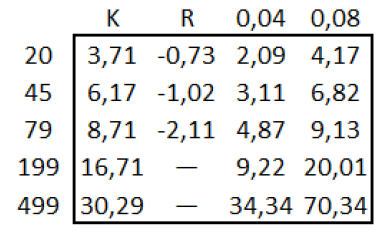
\includegraphics[width=0.42\textwidth]{poso-04.png}
% \par % так!!
% \caption{The main results of the computational experiments.}
% \mbox{\footnotesize Рис.~\arabic{ris-obho}. Об <<опоясывающем>> алгоритме.}
\label{table-1}
\end{table}

We think, that
the obtained results of computational experiments 
in general approximately correspond to the expected values.

\medskip

\textit{Acknowledgement.}
The work of the first author 
was partially supported by a grant 
from the scientific program of Chinese universities
``Higher Education Stability Support Program''
(section ``Shenzhen 2022~-- Science, Technology 
and Innovation Commission of Shenzhen Municipality'').

%
% ---- Bibliography ----
%
\begin{thebibliography}{5}

\bibitem{gu-pu}
Gutin, G., Punnen, A. (Eds.):
The traveling salesman problem and its variations.
Netherlands, Dordrecht: Kluwer Academic Publishers, 2002, 856~p.

\bibitem{KIO-2021}
Melnikov, B., Melnikova, E.
About the classical version of the branch and bound method.
Computer tools in education. 
2021. No.~1. Pp.~21-44 (in Russian).

\bibitem{KIO-2022}
Melnikov, B., Melnikova, E.
On the classical version of the branch and bound method.
Computer tools in education. 
2022. No.~2. Pp.~41-58.

\bibitem{Vasil-2022-1}
Melnikov, B.
On the object-oriented implementation
of the branch and bound method 
for the traveling salesman problem. Part I.
Modern information technologies and IT education. 
2022. Vol.~18. No.~2. Pp.~287-299 (in Russian).

\bibitem{Vasil-2022-2}
Melnikov, B.
On the object-oriented implementation
of the branch and bound method 
for the traveling salesman problem. Part II.
Modern information technologies and IT education. 
2022. Vol.~18. No.~3. Pp.~644-654 (in Russian).

\bibitem{SOI-2013}
Makarkin, S., Melnikov, B.
Geometric methods for solving the pseudo-geometric version 
of the traveling salesman problem.
Stochastic optimization in computer science. 
2013. Vol.~9. No.~2. Pp.~54-72 (in Russian).
\end{thebibliography}

%\end{document}  